Exact algorithms for the TSP are methods that guarantee finding the optimal solution to the problem by exploring all possible combinations of city tours. These algorithms are based on exhaustive search and systematic enumeration, ensuring that no potential solution is overlooked. While they may work well for small instances of the TSP, they become computationally infeasible for larger problem sizes since it leads to a time complexity of $O(n!)$.


\section{Benders}
Benders' Decomposition is a powerful optimization technique used to solve large-scale combinatorial problems like the Traveling Salesman Problem (TSP). It was introduced by Jacques F. Benders in the 1960s and has since become a widely used approach in the field of mathematical programming.

The Traveling Salesman Problem is known to be a challenging NP-hard problem, meaning that finding the optimal solution for large instances can be computationally intractable using traditional methods like brute-force or exact algorithms. Benders' Decomposition addresses this issue by breaking down the problem into smaller, more manageable subproblems and solving them iteratively.

The basic idea behind Benders' Decomposition is to partition the original problem into a master problem and multiple subproblems. The master problem is an integer linear programming (ILP) relaxation of the original TSP, allowing for the relaxation of some constraints. It aims to find a lower bound on the optimal solution value of the TSP. The subproblems, also known as \textit{Benders' cuts} or \textit{feasibility cuts}, are used to correct the solution obtained from the master problem by adding additional constraints that remove infeasible solutions, called \textit{Subtour Elimination Constraint} (SEC).

\begin{equation*}
    \sum_{e \in E(S_k)} x_e \leq |S_k|-1 \quad \quad \forall S_k: k=1,2,...
\end{equation*}

In our implementation \ref{algo:benders} we use CPLEX to build an initial ILP model of the TSP instance with only the degree equals 2 constraints for each node. We solve this model iteratively to obtain a solution,  which may not be feasible for the original TSP, in the sense that it contains subtours (internal cycles). Each subtour is considered a connected component and we generate Benders' cuts based on these components to eliminate them from consideration in subsequent iterations of the algorithm. We add these cuts to the CPLEX model, called \textit{Subtour Elimination Constraint} (SEC), which tightens the relaxation and improves the solution quality.



\begin{algorithm}
    \caption{Benders Algorithm}\label{algo:benders}
    \begin{algorithmic}[1]
    \Require $G = (V,E), c:E \to \mathbb{R}^+$
    \Ensure $\text{Optimal TSP solution}$
    
    \State $*$ initialize a basic CPLEX model with degree constraints $*$

    \State $ ncomp \gets 0$

    \While{$ !time_{expired} $}

        \State $*$ Solve CPLEX model$*$
        \State $ncomp \gets $ number of connected components

        \If{$ncomp = 1$}
            \State $*$ we found the optimal solution $*$
            \State \Return Solution
        \EndIf

        \State $*$ computes Patching Heuristic $*$

        \ForEach{connected component}

        \State $*$ add SEC $*$

        \EndFor

       

    \EndWhile

    \State \Return best Solution found


    \end{algorithmic}
\end{algorithm}

\subsection{Patching Heuristic}
In the Algorithm \ref{algo:benders} at line 10, we compute the Patching Heuristic.
It is an extension of Benders' Decomposition that aims to improve the quality of solutions obtained by the original Benders' algorithm before it terminates. 

It addresses a limitation of Benders' Decomposition, which may produce solutions with a relatively large optimality gap due to the relaxation of the TSP constraints in the master problem. The patching heuristic helps close this gap by iteratively improving the solution through additional modifications.

At each iteration of Benders, a solution is obtained, but it might still contain subtours due to the relaxation of constraints. The Patching Heuristic aims to identify and remove these subtours from the solution, thus achieving a feasible solution with tighter bound on the optimal solution value.

In our implementation, the Patching Heuristic repairs the current solution with subtours one component at a time until all components are connected. 
Starting from component number 1, it tries to find the edge that connect this component to a different one with lowest $\Delta$ (as defined in Equation \ref{eq:delta}) and then merges the two components. This process is repeated until all components are merged into one.

\begin{figure}[!h]
    \centering
    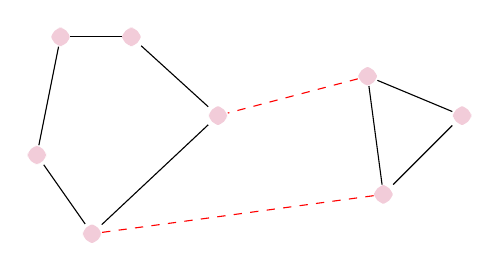
\begin{tikzpicture}
        \tikzstyle{city} = [fill=purple!20,rounded corners]


        \node[city] (A) at (2.3,5.0){};
        \node[city] (B) at (2.6,6.5){};
        \node[city] (C) at (7.7,5.5){};
        \node[city] (D) at (6.7,4.5){};
        \node[city] (E) at (3.0,4.0){};
        \node[city] (F) at (3.5,6.5){};
        \node[city] (G) at (4.6,5.5){};
        \node[city] (H) at (6.5,6){};


        %\draw[->] (C.west) -- (E.east);
        %\draw[->] (B.south) -- (A.east);
        \draw[] (C) edge (D) (E) edge (A) (A) edge (B) (B) edge (F) (F) edge (G) (G) edge (E) (D) edge (H) (H) edge (C);

        \draw[dashed, red] (D) edge (E) (H) edge (G);

    \end{tikzpicture}
    \caption{Example of Patching Heuristic} \label{fig:patch}
\end{figure}





\section{Concorde}

\subsection{Tuning of Concorde}

\section{Comparison of Exact Methods}